\documentclass[a4paper,12pt]{extarticle}
\usepackage{geometry}
\usepackage[T1]{fontenc}
\usepackage[utf8]{inputenc}
\usepackage[english,russian]{babel}
\usepackage{amsmath}
\usepackage{amsthm}
\usepackage{amssymb}
\usepackage{fancyhdr}
\usepackage{setspace}
\usepackage{graphicx}
\usepackage{colortbl}
\usepackage{tikz}
\usepackage{pgf}
\usepackage{subcaption}
\usepackage{listings}
\usepackage{indentfirst}
\usepackage[
backend=biber,
style=numeric,
maxbibnames=99
]{biblatex}
\addbibresource{references.bib}
\usepackage[colorlinks,citecolor=blue,linkcolor=blue,bookmarks=false,hypertexnames=true, urlcolor=blue]{hyperref} 
\usepackage{indentfirst}
\usepackage{mathtools}
\usepackage{booktabs}
\usepackage[flushleft]{threeparttable}
\usepackage{tablefootnote}

\usepackage{chngcntr} % нумерация графиков и таблиц по секциям
\counterwithin{table}{section}
\counterwithin{figure}{section}

\graphicspath{{graphics/}}%путь к рисункам

\makeatletter
% \renewcommand{\@biblabel}[1]{#1.} % Заменяем библиографию с квадратных скобок на точку:
\makeatother

\geometry{left=2.5cm}% левое поле
\geometry{right=1.0cm}% правое поле
\geometry{top=2.0cm}% верхнее поле
\geometry{bottom=2.0cm}% нижнее поле
\setlength{\parindent}{1.25cm}
\renewcommand{\baselinestretch}{1.5} % междустрочный интервал


\newcommand{\bibref}[3]{\hyperlink{#1}{#2 (#3)}} % biblabel, authors, year
\addto\captionsrussian{\def\refname{Список литературы (или источников)}} 

\renewcommand{\theenumi}{\arabic{enumi}}% Меняем везде перечисления на цифра.цифра
\renewcommand{\labelenumi}{\arabic{enumi}}% Меняем везде перечисления на цифра.цифра
\renewcommand{\theenumii}{.\arabic{enumii}}% Меняем везде перечисления на цифра.цифра
\renewcommand{\labelenumii}{\arabic{enumi}.\arabic{enumii}.}% Меняем везде перечисления на цифра.цифра
\renewcommand{\theenumiii}{.\arabic{enumiii}}% Меняем везде перечисления на цифра.цифра
\renewcommand{\labelenumiii}{\arabic{enumi}.\arabic{enumii}.\arabic{enumiii}.}% Меняем везде перечисления на цифра.цифра

\theoremstyle{definition}
\newtheorem{definition}{Определение}[section]

\theoremstyle{examples}
\newtheorem{examples}{Примеры}[section]

\begin{document}
\begin{titlepage}
\newpage

{\setstretch{1.0}
\begin{center}
ПРАВИТЕЛЬСТВО РОССИЙСКОЙ ФЕДЕРАЦИИ\\
ФГАОУ ВО НАЦИОНАЛЬНЫЙ ИССЛЕДОВАТЕЛЬСКИЙ УНИВЕРСИТЕТ\\
«ВЫСШАЯ ШКОЛА ЭКОНОМИКИ»
\\
\bigskip
Факультет компьютерных наук\\
Образовательная программа «Компьютерные науки и анализ данных»
\end{center}
}

\vspace{2em}
УДК 004.932:004.032.26:515.14 % обработка изображений + нейронные сети + алгебраическая топология
\vspace{4em}

\begin{center}
{\bf Отчет об исследовательском проекте на тему:}\\
{\bf Топологический анализ изображений}\\
% строчка ниже нужна только при сдача плана КР, при финальной сдаче закомментируйте ее
(промежуточный, этап 1)
\end{center}

\vspace{2em}

{\bf Выполнил студент: \vspace{2mm}}

{\setstretch{1.1}
\begin{tabular}{l@{\hskip 1.5cm}l}
группы \#БКНАД231, 3 курса & Мусалов Никита Сергеевич
\end{tabular}}

\vspace{1em}
{\bf Принял руководитель проекта: \vspace{2mm}}

{\setstretch{1.1}
\begin{tabular}{l}
Качан Олег Николаевич\\
Преподаватель\\
Факультет компьютерных наук НИУ ВШЭ 
\end{tabular}}

\vspace{\fill}

\begin{center}
Москва 2026
\end{center}

\end{titlepage}% это титульный лист - выберите подходящий вам из имеющихся в проекте вариантов (kr - курсовая работа у 3 курса, vkr - выпускная квалификационная работа у 4 курса)
\newpage
\setcounter{page}{2}

{
	\hypersetup{linkcolor=black}
	\tableofcontents
}

\newpage

\newpage
\section*{Аннотация}
Большинство цифровых изображений представляют из себя изображения на двумерной или трехмерной сетке, либо их временные ряды. Признаки извлекаемые методами топологического анализа данных являются новым классом признаков описывающих глобальную структуру изображений, в отличие от информации извлекаемой сверточными нейросетями и трансформерами. Такие топологические и геометрические признаки изображений как диаграмма устойчивости или функционалы Минковского могут быть извлечены не только из исходных изображений, но их преобразований различными фильтрами, параметры которых могут быть обучены по данным. Подобные методы находят применение для решения задач диагностики по данным радиологии и компьютерной томографии, сегментации медицинских изображений и изображений со спутников, а также оценки физических параметров пористых материалов.

\addcontentsline{toc}{section}{Аннотация}

\section*{Ключевые слова}
Топологический анализ данных, Глубинное обучение, Компьютерное зрение
\pagebreak

\section{Введение}
\begin{sloppypar}
    Топологический анализ данных (TDA) --- это быстро развивающаяся область, возникшая на основе различных работ в алгебраической топологии и вычислительной геометрии. Она предлагает набор методов для выявления глобальных характеристик пространственных данных, дополняющих признаки, извлекаемые классическими методами компьютерного зрения. В этом разделе мы кратко вводим необходимый аппарат TDA (§\ref{ssec:basic-defs}), затем обсуждаем его специализацию на цифровые изображения и важные для нашей работы направленные фильтрации (§\ref{ssec:tda-images}), и наконец формулируем задачу эмбеддинга диаграмм персистентности, которой посвящён остальной отчёт (§\ref{sec:embedding-task}).

\subsection{Базовые определения}
\label{ssec:basic-defs}
\begin{sloppypar}
    Под \emph{симплициальным комплексом} мы будем понимать конечный набор $K$ симплексов, замкнутый относительно взятия граней: если $\sigma \in K$ и $\tau \subseteq \sigma$, то $\tau \in K$. Симплициальный комплекс служит дискретным аналогом топологического пространства и базовым объектом, на котором будет считаться гомология.

Когда данные приходят в виде облака точек в метрическом пространстве, чтобы превратить их в симплициальный комплекс, обычно используют конструкцию комплекса Чеха.
\begin{definition}[Комплекс Чеха]
Пусть $(X, d)$ - метрическое пространство, $P \subseteq X$ - конечное множество, и $\varepsilon \ge 0$.
\emph{Комплексом Чеха} $\check{C}_{\varepsilon}(P)$ называется симплициальный комплекс с множеством вершин $P$, в котором
конечное подмножество $\sigma\subseteq P$ является симплексом тогда и только тогда, когда
\[
\bigcap_{p\in \sigma} B(p, \varepsilon) \neq \varnothing,
\]
где $B(p, \varepsilon)$ - открытый шар радиуса $\varepsilon$ с центром в точке $p$.
\end{definition}

Реальные данные обычно зашумлены, поэтому один комплекс Чеха, построенный по фиксированному масштабу $\varepsilon$, говорит о геометрии облака немного. Кроме того, каждая точка может нести дополнительную информацию (например, значение какой-то функции), которая в одиночном комплексе Чеха никак не учитывается. Чтобы преодолеть оба ограничения, вводится понятие фильтрации --- семейства комплексов, упорядоченных по шкале параметра.
\begin{definition}[Фильтрация]
Пусть $K$ --- симплициальный комплекс, а $(I,\le)$ --- частично упорядоченное множество.
\emph{Фильтрацией} комплекса $K$, индексированной $I$, называется семейство симплициальных подкомплексов
$\{K_\alpha\}_{\alpha\in I}$, где $K_\alpha\subseteq K$, такое что для любых $\alpha\le \beta$ выполнено
\[
K_\alpha \subseteq K_\beta.
\]
Мы будем брать $I=\mathbb{R}$ или $I=\mathbb{Z}$ с обычным порядком.
\end{definition}

\begin{examples}
Приведем важнейшие примеры фильтраций
\begin{itemize}
\item Семейство комплексов Чеха $\{\check{C}_{\varepsilon}(P)\}_{\varepsilon \ge 0}$, параметризованное $\varepsilon \in \mathbb{R}_{\ge 0}$, является фильтрацией: из $\varepsilon \le \varepsilon'$ следует $\check{C}_{\varepsilon}(P)\subseteq \check{C}_{\varepsilon'}(P)$.
Такой объект даёт значительно более репрезентативное представление облака точек, чем комплекс Чеха с фиксированным масштабом.

\item Фильтрация по подуровням функции.
Пусть $K$ - симплициальный комплекс с множеством вершин $V$, и пусть задана функция $w:V\to\mathbb{R}$.
Продлим её на симплексы по правилу
\[
w(\sigma) := \max_{v\in\sigma} w(v).
\]
Для $a\in\mathbb{R}$ положим
\[
K_a := \{\sigma\in K : w(\sigma)\le a\}.
\]
Тогда каждое $K_a$ является симплициальным подкомплексом, и $\{K_a\}_{a\in\mathbb{R}}$ образует фильтрацию комплекса $K$. Это позволяет учитывать скрытое представление каждой точки. Например, изображение как облако пикселей в плоскости само по себе малоинформативно, но если задать функцию из каждого пикселя в его яркость и построить по ней фильтрацию по подуровням, мы получим осмысленное топологическое описание изображения.
\end{itemize}
\end{examples}

% \begin{definition}[Симплициальные гомологии]
% Пусть $K$ - симплициальный комплекс. Для $k\ge 0$ определим $\Bbbk$-векторное пространство $k$-цепей:
% \[
% C_k(K;\Bbbk) := \bigoplus_{\sigma\in K_k} \Bbbk\cdot \sigma,
% \]
% то есть свободное $\Bbbk$-пространство, порождённое (ориентированными) $k$-симплексами.
% Граничный оператор $\partial_k: C_k(K;\Bbbk)\to C_{k-1}(K;\Bbbk)$ задаётся на порождающих формулой
% \[
% \partial_k [v_0,\dots,v_k] := \sum_{i=0}^k (-1)^i [v_0,\dots,\widehat{v_i},\dots,v_k],
% \]
% и продолжается $\Bbbk$-линейно. Выполнено $\partial_{k-1}\circ\partial_k=0$.
% Определим пространства циклов и границ:
% \[
% Z_k(K;\Bbbk):=\ker(\partial_k),\qquad B_k(K;\Bbbk):=\operatorname{im}(\partial_{k+1}).
% \]
% Тогда $k$-я симплициальная группа гомологий равна
% \[
% H_k(K;\Bbbk) := Z_k(K;\Bbbk)/B_k(K;\Bbbk).
% \]
% \end{definition}

\begin{definition}[Персистентные гомологии]
Пусть $\{K_a\}_{a \in I}$ --- фильтрация, индексированная линейно упорядоченным множеством $(I, \le)$, и пусть $n \ge 0$.
Для $a\le b$ включение $K_a\hookrightarrow K_b$ индуцирует гомоморфизм цепных комплексов и, соответственно, линейное отображение гомологий:
\[
f^{(n)}_{a\le b}: H_n(K_a;\Bbbk)\to H_n(K_b;\Bbbk).
\]
\emph{$n$-й персистентной гомологией} от $a$ к $b$ называется образ
\[
H_n^{a\to b}(\{K_\alpha\}_{\alpha \in I};\Bbbk) := \operatorname{Im}\bigl(f^{(n)}_{a\le b}\bigr)\subseteq H_n(K_b;\Bbbk).
\]
Эквивалентно,
\[
H_n^{a\to b} \cong \frac{Z_n(K_a;\Bbbk)}{Z_n(K_a;\Bbbk)\cap B_n(K_b;\Bbbk)}.
\]
Система $\{H_n(K_a;\Bbbk), f^{(n)}_{a\le b}\}_{a\le b \in I}$ называется $n$-м персистентным модулем фильтрации $\{K_a\}_{a \in I}$.
\end{definition}

\begin{definition}[Диаграмма персистентности]
В случае $I = \{0, 1, \dots, N\}$ прямую сумму $\bigoplus_{a \in I} H_n(K_a, \Bbbk)$ можно рассматривать как модуль над кольцом $\Bbbk[t]$, где действие $t$ задаётся правилом
\[
v \in H_n(K_a; \Bbbk), \quad t \cdot v = f^{(n)}_{a \le a+1}(v).
\]
Тогда по структурной теореме о конечно порождённых модулях над областями главных идеалов он раскладывается в прямую сумму интервальных модулей вида $[b_i, d_i)$, где $b_i < d_i \le \infty$.

\emph{$n$-й диаграммой персистентности} $\mathrm{Dgm}_n$ называется мультимножество точек
\[
\mathrm{Dgm}_n := \{(b_i, d_i)\}_i \subseteq \overline{\mathbb{R}}^2, \qquad \overline{\mathbb{R}} := \mathbb{R} \cup \{\infty\},
\]
взятое с кратностями, соответствующее интервалам в указанном разложении. Точки вблизи диагонали $b = d$ принято считать шумом, тогда как точки с большой персистентностью $d - b$ отвечают устойчивым топологическим признакам.
\end{definition}

    \hspace{1cm}
\end{sloppypar}

\subsection{TDA на изображениях}
\label{ssec:tda-images}
\begin{sloppypar}
    Цифровое изображение естественно рассматривать как функцию на пиксельной сетке: $I: \{1, \dots, H\} \times \{1, \dots, W\} \to \mathbb{R}$, где значение $I(p)$ интерпретируется как яркость (для одноканальных изображений) или один из каналов цвета. Чтобы применить к нему аппарат персистентных гомологий, нужно (а) задать симплициальный комплекс $K$, отражающий геометрию решётки, и (б) определить на нём фильтрацию, согласованную с содержимым изображения. В качестве $K$ обычно берут кубический комплекс, в котором симплексами являются пиксели (нульмерные клетки), их рёбра (одномерные клетки), сцепляющие соседние пиксели, и квадраты (двумерные клетки), заполняющие промежутки между четвёрками соседей. Этот выбор естественен и хорошо поддерживается современными вычислительными библиотеками.

\paragraph{Подуровневая фильтрация по интенсивности.}
Простейшая фильтрация на изображении --- подуровневая по самой интенсивности. Положим $w(p) = I(p)$ и распространим $w$ на симплексы по правилу $w(\sigma) = \max_{p \in \sigma} w(p)$ (см.\ §\ref{ssec:basic-defs}). Семейство подкомплексов
\[
K_a = \{\sigma \in K : w(\sigma) \le a\}, \qquad a \in \mathbb{R},
\]
образует фильтрацию, отражающую <<рост>> области тёмных пикселей при увеличении порога $a$. Соответствующая диаграмма $\mathrm{Dgm}_0$ кодирует появление и исчезновение связных компонентов уровня, а $\mathrm{Dgm}_1$ --- появление и заполнение петель (одномерных дыр), что для изображения отпечатка пальца, к примеру, отвечает гребням и впадинам узора.

\paragraph{Направленные фильтрации и Persistent Homology Transform.}
Подуровневая фильтрация по интенсивности использует только значения функции и игнорирует пространственную ориентацию структур на изображении. Чтобы исправить это, в работе Turner, Mukherjee, Boyer (2014)~\cite{turnerPersistentHomologyTransform2014} было предложено рассматривать целое семейство направленных фильтраций, индексированных направлениями. Для каждого единичного вектора $v_\alpha = (\cos\alpha, \sin\alpha)$, $\alpha \in [0, 2\pi)$, определим функцию высоты
\[
w_\alpha(p) = \langle p, v_\alpha \rangle = p_x \cos\alpha + p_y \sin\alpha,
\]
и по ней построим подуровневую фильтрацию. Получающееся отображение
\[
\mathrm{PHT}: \alpha \mapsto \bigl( \mathrm{Dgm}_0(\alpha), \mathrm{Dgm}_1(\alpha) \bigr)
\]
называется \emph{Persistent Homology Transform} (PHT) и для кусочно-линейных поверхностей в $\mathbb{R}^2$/$\mathbb{R}^3$ является инъективным: знание диаграмм во всех направлениях позволяет восстановить форму объекта~\cite{turnerPersistentHomologyTransform2014}. Это делает PHT богатым по информации топологическим дескриптором формы, чувствительным к ориентации, в отличие от чисто радиально-симметричных характеристик.

На практике непрерывное семейство $\alpha \in [0, 2\pi)$ дискретизируется конечным набором направлений. В нашей реализации (см.\ \texttt{src/filtrations/pht.py}) по умолчанию используется $16$ равномерно распределённых углов $\alpha \in \{0^\circ, 22{.}5^\circ, \dots, 337{.}5^\circ\}$. Для каждого направления получается своя диаграмма с точками вида $(b, d)$; объединение всех таких диаграмм и составляет вход для модели. Чтобы модель могла различать диаграммы из разных направлений, к каждой точке прикрепляется метаинформация: гомологическая размерность, флаг типа фильтрации (sublevel/PHT), сам угол $\alpha$ и его синусоидальное позиционное кодирование. Таким образом, одна точка диаграммы превращается в небольшой вектор признаков, что естественным образом подаётся в нейронные сети, обрабатывающие неупорядоченные множества (см. §\ref{sec:embedding-task}).

\begin{figure}[ht]
\centering
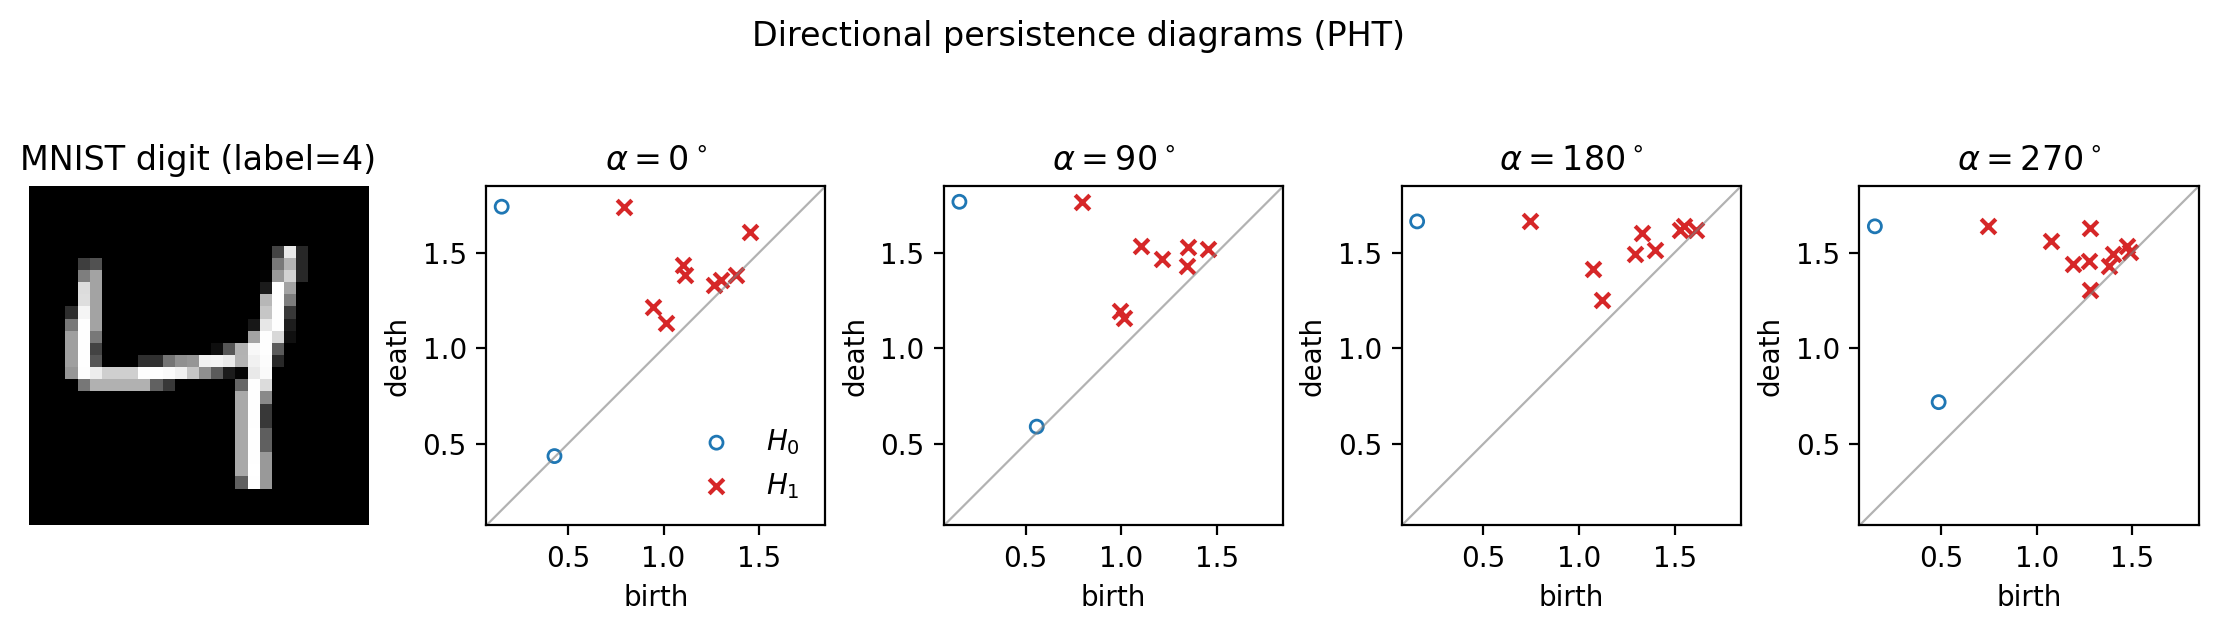
\includegraphics[width=\linewidth]{figures/mnist_directional_pht.png}
\caption{Пример изображения цифры из MNIST (слева) и соответствующие диаграммы персистентности, получаемые направленной фильтрацией для четырёх направлений $\alpha \in \{0^\circ, 90^\circ, 180^\circ, 270^\circ\}$ (справа). Точки $H_0$ и $H_1$ изображены разными маркерами; видно, как направление фильтрации перераспределяет точки между диаграммами и тем самым кодирует ориентацию структур на изображении.}
\label{fig:pht-illustration}
\end{figure}

    \hspace{1cm}
\end{sloppypar}

\subsection{Задача эмбеддинга TDA-признаков}
\begin{sloppypar}
    \label{sec:embedding-task}
Описанный в §1.2 пайплайн выдаёт для каждого изображения набор диаграмм персистентности --- по одной на каждое направление PHT-фильтрации, плюс, при желании, отдельную диаграмму подуровневой фильтрации. Чтобы использовать эти диаграммы в задачах классификации и регрессии, их нужно превратить в признаки, совместимые с алгоритмами машинного обучения. Эта и составляет \emph{задачу эмбеддинга} диаграмм персистентности.

\paragraph{Почему задача нетривиальна.}
Диаграмма персистентности $D$ --- это \emph{мультимножество} точек переменной мощности в $\mathbb{R}^2 \cup (\mathbb{R} \times \{\infty\})$. У такого объекта есть три свойства, затрудняющих прямое использование стандартных моделей:
\begin{enumerate}
\item \emph{Переменный размер}: разные изображения порождают разное число точек в диаграмме, тогда как большинство ML-методов требует входа фиксированной размерности.
\item \emph{Перестановочная инвариантность}: диаграмма как множество не имеет естественного порядка, и любой эмбеддинг $\phi(D)$ должен быть инвариантен к перестановке точек.
\item \emph{Невозможность изометрического вложения в гильбертово пространство}: пространство диаграмм с метрикой Вассерштейна, как показано в работах~\cite{mileykoProbabilityMeasuresSpace2011}, не вкладывается изометрически ни в какое гильбертово пространство. Это означает, что прямое использование диаграммы как точки в евклидовом пространстве не сохраняет геометрию пространства диаграмм; искажение неизбежно.
\end{enumerate}

\paragraph{Формальная постановка.}
Будем искать отображение $\phi: \mathcal{D} \to \mathbb{R}^n$ (или в гильбертово пространство $\mathcal{H}$), где $\mathcal{D}$ --- пространство диаграмм персистентности, удовлетворяющее набору желательных свойств:
\begin{itemize}
\item[(i)] \textbf{Фиксированная размерность.} Выход $\phi(D)$ --- вектор фиксированной длины, не зависящей от числа точек в $D$.
\item[(ii)] \textbf{Перестановочная инвариантность.} $\phi(D) = \phi(\pi \cdot D)$ для любой перестановки точек $\pi$ диаграммы $D$.
\item[(iii)] \textbf{Устойчивость.} Небольшое возмущение входа (в смысле метрики Вассерштейна на $\mathcal{D}$) приводит к небольшому изменению $\phi(D)$.
\item[(iv)] \textbf{Дифференцируемость} по обучаемым параметрам $\phi_\theta$, что позволяет интегрировать эмбеддинг в end-to-end обучаемые pipelines.
\item[(v)] \textbf{Достаточная выразительность} для конкретной задачи --- т.\,е. способность аппроксимировать произвольную непрерывную функцию на $\mathcal{D}$ (универсальная аппроксимация).
\end{itemize}

\paragraph{Два класса методов.}
В литературе сложилось два больших семейства подходов к эмбеддингу диаграмм:
\begin{itemize}
\item \emph{Предписанные (prescribed) представления} --- $\phi$ задаётся аналитически и не имеет обучаемых параметров. Такие методы, как правило, обладают доказанной устойчивостью и легко интерпретируемы, но не настраиваются под конкретную задачу и теряют информацию в шагах дискретизации и при выборе весовой функции. Типичные представители: persistence image~\cite{adamsPersistenceImages2017}, persistence landscape~\cite{bubenikStatisticalTopologicalData2015}, persistence silhouette~\cite{chazalStochasticConvergencePersistence2014}.
\item \emph{Обучаемые (learned) представления} --- $\phi_\theta$ параметризовано нейронной сетью, обученной совместно с downstream-задачей. Сюда относятся DeepSets~\cite{zaheerDeepSets2017}, PersLay и Persformer~\cite{reinauerPersformerTransformerArchitecture2021}. Они более выразительны и адаптивны, но требуют значительно больше данных и вычислений.
\end{itemize}

\paragraph{Особенности нашей постановки.}
В нашей работе вход усложняется тем, что для одного изображения формируется набор диаграмм по 16 направлениям PHT (а иногда плюс подуровневая фильтрация). С точки зрения эмбеддинга это означает, что:
\begin{itemize}
\item каждая точка приходит с метаинформацией о направлении $\alpha$ и о типе фильтрации, и эмбеддинг должен уметь использовать эту информацию;
\item общее число точек на одно изображение становится большим (сотни и тысячи), что вносит требования по масштабируемости в число точек;
\item инвариантность нужна именно по перестановкам внутри объединённого мультимножества, не по полностью независимым диаграммам.
\end{itemize}
Эти соображения и формируют требования к предлагаемой в §3 архитектуре. В §2 мы сначала разберём, как существующие методы эмбеддинга решают перечисленные критерии (i)--(v), а затем обсудим, где они оказываются недостаточны для нашего сценария.

    \hspace{1cm}
\end{sloppypar}

\subsection{Датасеты и постановка задачи}
\begin{sloppypar}
    В первой задаче требуется по изображению отпечатка пальца предсказать его класс по классификации Генри. Для обучения и оценки используется несколько датасетов:
\begin{itemize}
\item NIST Special Database 4~\cite{NIST-SD-4} - основной датасет. Используется как базовый источник примеров отпечатков для обучения модели предсказанию классов по Генри и для корректного сравнения с работами, опирающимися на стандартизованные наборы NIST.
\item SokoFING~\cite{SOCOFing} - дополнительный датасет. Его полезно использовать в двух режимах: (a) как дополнительный источник обучения (совместно с NIST SD4); (b) как внешний тест, чтобы проверить переносимость модели за пределы основного датасета.
\item Fingerprint Minutiae Computer Vision Dataset~\cite{fingerprint-minutiae-dataset} - датасет c картами минуций. Используется для построения модели, которая будет применяться на этапе предобработки для построения карты направленных минуций. Основная модель будет проводить классификацию уже с использованием карты минуций. 
\item CASIA-FingerprintV5~\cite{CASIA-fingerprintV5} - дополнительный большой датасет для претрейна в self-supervised режиме.
\end{itemize}


Во второй задаче требуется предсказать определенные свойства пористых материалов, в частности, металл-органических каркасных структур (MOF). Чаще всего рассматриваются адсорбционные свойства: например, способность данного MOF поглощать определенный газ при разных давлениях. Ключевой особенностью будет использование топологических дескрипторов, извлечённых из структуры порового пространства материала, в качестве признаков для модели. Для обучения и оценки моделей планируется использовать несколько наборов данных MOF:

\begin{itemize}
\item Hypothetical MOFs~\cite{Wilmer2012} – база гипотетических структур MOF. Этот датасет содержит структуры (54k материалов) из MOFXDB и рассчитанные характеристики адсорбции $\text{CO}_2$ при пяти различных давлениях.
\item Boyd–Woo MOF~\cite{Boyd-Woo} – база предсказанных структур MOF. В этот набор входят рассчитанные показатели адсорбции метана и $\text{CO}_2$ при низком и высоком давлениях, а также коэффициенты Генри для этих газов.
\item CoRE MOF 2019~\cite{CoreMOF2019} – подборка экспериментально синтезированных структур MOF из базы CoRE MOF. Она представляет реальные пористые материалы, пригодные для оценки обобщающей способности моделей.
\end{itemize}


В третьей задаче рассматривается семантическая сегментация медицинских изображений - автоматическое разделение изображения на области, соответствующие различным анатомическим структурам. Акцент делается на топологически корректной сегментации, то есть предсказанные области должны иметь количество связных компонентов и отверстий, совпадающее с анатомически правильным . Для этого планируется встроить сравнение топологических характеристик в лосс при обучении модели. Для обучения и оценки моделей планируется использовать датасет:

\begin{itemize}
\item AMOS~\cite{ji2022amos,amos2022zenodo} - клинический датасет для 3D-сегментации органов брюшной полости на КТ и МРТ. Он включает 600 исследований на 600 пациентах (500 КТ и 100 МРТ), содержит воксельную разметку 15 органов (включая селезёнку, печень, почки, поджелудочную железу, аорту и др.).
\end{itemize}

    \hspace{1cm}
\end{sloppypar}

    \hspace{1cm}
\end{sloppypar}

\section{Обзор литературы}
\begin{sloppypar}
    В этом разделе мы последовательно разбираем основные подходы к эмбеддингу диаграмм персистентности: сначала три классические предписанные конструкции (Persistence Image, Persistence Landscape, Persistence Silhouette), затем два обучаемых подхода (DeepSets и Persformer). Для каждого метода мы кратко описываем устройство, сильные стороны и ограничения с точки зрения сформулированных в §\ref{sec:embedding-task} критериев (i)--(v).

\subsection{Persistence Image}
\label{ssec:pi}

Persistence Image~\cite{adamsPersistenceImages2017} превращает диаграмму $D$ в небольшое <<изображение>> --- двумерную карту значений на регулярной сетке. Сначала диаграмма переводится из координат \emph{birth--death} в координаты \emph{birth--persistence} линейным преобразованием $T(b, d) = (b, d - b)$, после чего по преобразованной диаграмме $T(D)$ строится \emph{поверхность персистентности}:
\[
\rho_D(z) = \sum_{u \in T(D)} f(u) \cdot \phi_u(z),
\]
где $\phi_u$ --- нормированный гауссиан с центром $u$ и фиксированной дисперсией $\sigma^2$, а $f \colon \mathbb{R}^2 \to \mathbb{R}_{\ge 0}$ --- весовая функция, равная нулю на горизонтальной оси (соответствующей диагонали $b = d$) и плавно растущая с увеличением persistence. Persistence image $I(D)$ получается дискретизацией поверхности по равномерной сетке размера $n \times n$ и интегрированием $\rho_D$ по каждой ячейке.

Persistence Image удовлетворяет критериям (i), (ii) и (iii): результат --- вектор фиксированного размера $n^2$, инвариантный по перестановкам точек, а 1-Wasserstein-устойчивость относительно вариаций входа доказана авторами. К ограничениям относятся: необходимость подбирать резолюцию $n$, дисперсию $\sigma^2$ и весовую функцию $f$ под задачу (теряется адаптивность); отсутствие моделирования взаимодействий между точками --- влияние каждой точки <<суммируется>> аддитивно; результат лежит в евклидовом пространстве, но не настраивается под downstream-задачу.

\subsection{Persistence Landscape}
\label{ssec:pl}

Persistence Landscape~\cite{bubenikStatisticalTopologicalData2015} представляет диаграмму как набор кусочно-линейных функций. Для каждой точки $(b_i, d_i)$ диаграммы определяется <<шапочка>>
\[
f_{(b_i, d_i)}(x) = \max\bigl(0, \min(x - b_i, d_i - x)\bigr),
\]
а ландшафт уровня $k$ --- это огибающая $k$-й по убыванию функции:
\[
\lambda_k(x) = \mathop{\mathrm{kmax}}_{i} f_{(b_i, d_i)}(x),
\]
где $\mathop{\mathrm{kmax}}$ обозначает $k$-е по убыванию значение. Ландшафт $\lambda = (\lambda_1, \lambda_2, \dots)$ лежит в $L^p$-Банаховом пространстве, что делает его удобным для статистических процедур: средние, доверительные интервалы и ядра определяются естественно. На практике первые $K$ слоёв оцениваются на равномерной сетке из $R$ точек, что даёт вектор фиксированной длины $K \cdot R$.

Главные преимущества landscape --- наличие сильной теории устойчивости (по $L^\infty$-норме и относительно bottleneck-расстояния) и линейность по диаграммам, позволяющая корректно усреднять. Ограничения схожи с PI: эмбеддинг не имеет обучаемых параметров; число слоёв $K$ и резолюция $R$ выбираются вручную; представление сужается, когда у диаграмм много <<близких>> точек --- они обмениваются местами на разных слоях и могут создавать высокочастотные артефакты.

\subsection{Persistence Silhouette}
\label{ssec:ps}

Persistence Silhouette~\cite{chazalStochasticConvergencePersistence2014} сглаживает диаграмму до единственной функции одной переменной --- взвешенного среднего тех же шапочек $f_{(b_i, d_i)}$:
\[
\phi^{(p)}(x) = \frac{\sum_i |d_i - b_i|^p \cdot f_{(b_i, d_i)}(x)}{\sum_i |d_i - b_i|^p},
\]
где параметр $p \ge 0$ управляет относительным весом высоко- и низкопересистентных точек: при $p \to 0$ все точки учитываются равноправно, при $p \to \infty$ доминируют наиболее значимые. Дискретизация на $R$ узлов сетки даёт вектор фиксированной длины $R$.

Silhouette гораздо компактнее ландшафта (одна функция вместо $K$ слоёв), сохраняет статистическую трактовку и устойчивость, но при этом теряет часть информации о структуре диаграммы --- в частности, не позволяет различить ситуацию с одной значимой точкой от ситуации с несколькими равноценными. Как и landscape, не обучается под задачу.

\subsection{DeepSets}
\label{ssec:deepsets}

DeepSets~\cite{zaheerDeepSets2017} --- общая конструкция для построения перестановочно-инвариантных функций на множествах. Утверждение состоит в том, что любую непрерывную перестановочно-инвариантную функцию на множествах ограниченного размера можно сколь угодно точно приблизить выражением
\[
L(\{x_1, \dots, x_n\}) = \rho \!\left( \sum_{i=1}^{n} \phi(x_i) \right),
\]
где $\phi$ и $\rho$ --- нейронные сети (обычно MLP). В применении к диаграммам персистентности роль $x_i$ играют точки $(b_i, d_i)$ (возможно, с одношаговым one-hot-кодированием гомологической размерности): $\phi$ применяется к каждой точке независимо, результаты симметрично агрегируются (суммой или средним, в реализации часто с маской для padding'а), и итог пропускается через декодирующий MLP $\rho$.

DeepSets обучаема, перестановочно-инвариантна, дифференцируема и масштабируется линейно по числу точек. Главное её ограничение --- отсутствие явного моделирования \emph{взаимодействий} между точками: каждая точка обрабатывается изолированно, а вся <<коммуникация>> сводится к одному pooling-шагу. Для диаграмм, где относительное расположение точек несёт сигнал (например, кластеризация близких к диагонали точек или линейное расположение точек одного и того же масштаба), это становится бутылочным горлышком.

\subsection{Persformer}
\label{ssec:persformer}

Persformer~\cite{reinauerPersformerTransformerArchitecture2021} --- наиболее <<современный>> по архитектуре из рассмотренных подходов. Точки диаграммы трактуются как множество векторов в $\mathbb{R}^2$ (расширенное one-hot-кодированием гомологической размерности), к ним применяется обучаемое позиционное кодирование (линейный input embedding), затем стек self-attention блоков из стандартного трансформера, и наконец --- multi-head attention pooling layer с единственной обучаемой query~\cite{leeSetTransformer2019} для получения вектора фиксированного размера. Полученный вектор обрабатывается небольшим MLP-классификатором.

Главное достоинство Persformer --- self-attention механизм моделирует попарные взаимодействия между всеми точками диаграммы и, как показано авторами, удовлетворяет универсальной аппроксимационной теореме для функций на мультимножествах. Это снимает основное ограничение DeepSets. Кроме того, благодаря saliency maps Persformer допускает интерпретацию: можно оценивать вклад каждой точки диаграммы в финальное предсказание.

Главные ограничения связаны с вычислительной стоимостью: вычислительная сложность self-attention квадратична по числу точек $M$ во входе, $O(M^2)$. Для диаграмм из 30--50 точек это не проблема, однако в нашей задаче с PHT-фильтрацией по 16 направлениям одно изображение порождает сотни и тысячи токенов, и квадратичная сложность становится узким местом и по памяти, и по времени.

\subsection{Сводка}
Таблица~\ref{tab:methods-summary} обобщает сравнение по сформулированным критериям. Видно, что предписанные методы дёшевы и устойчивы, но негибки; DeepSets и Persformer обучаемы и выразительны, но различаются по способности моделировать взаимодействия и по масштабируемости. Именно поиск точки компромисса в треугольнике <<выразительность $\leftrightarrow$ сложность $\leftrightarrow$ масштабируемость>>, с учётом особенностей нашей PHT-постановки, мотивирует архитектуру, описанную в §3.

\begin{table}[ht]
\centering
\fbox{\parbox{0.85\linewidth}{\centering [PLACEHOLDER]\\[0.3em]
Сводная таблица: для каждого метода (PI, PL, PS, DeepSets, Persformer) --- столбцы <<обучаемость>>, <<взаимодействия между точками>>, <<сложность по числу точек $M$>>, <<доказанная устойчивость>>, <<интерпретируемость>>.}}
\caption{Сравнение методов эмбеддинга диаграмм персистентности.}
\label{tab:methods-summary}
\end{table}

    \hspace{1cm}
\end{sloppypar}

\newpage 
\printbibliography[heading=bibintoc] 

\end{document}
